% !TeX program = xelatex
\documentclass[aspectratio=169,11pt]{beamer}

\usetheme{metropolis}
\metroset{block=fill,progressbar=frametitle,numbering=fraction,sectionpage=progressbar}

\usepackage{amsmath,amssymb}
\usepackage{booktabs}
\usepackage{graphicx}
\usepackage{tikz}
\usepackage{enumitem}
\usetikzlibrary{positioning}

\setlist{itemsep=3pt,topsep=2pt,parsep=0pt}

\definecolor{nanogune}{RGB}{0,96,153}
\setbeamercolor{palette primary}{bg=nanogune,fg=white}
\setbeamercolor{titlelike}{fg=nanogune}
\setbeamercolor{frametitle}{bg=nanogune,fg=white}
\setbeamercolor{progress bar}{fg=nanogune,bg=nanogune!20}
\setbeamercolor{alerted text}{fg=red!65!black}
\setbeamercolor{block title}{bg=nanogune!85!black,fg=white}
\setbeamercolor{block body}{bg=nanogune!8}
\setbeamercolor{block title alerted}{bg=red!65!black,fg=white}
\setbeamercolor{block body alerted}{bg=red!6}
\setbeamerfont{block title}{size=\small}
\setbeamerfont{block body}{size=\small}
\setbeamerfont{block title alerted}{size=\small}
\setbeamerfont{block body alerted}{size=\small}

\graphicspath{{figs/}}

\title{Emergent Magnetism in Finite Nanographenes}
\subtitle{Topological end states in 7-AGNRs and a designed Heisenberg spin chain in triangulene--phenalenyl copolymers}
\author{L.~Zulueta}
\institute{CIC nanoGUNE, Donostia--San Sebasti\'an, Spain}
\date{\today}

\begin{document}

\maketitle

\begin{frame}{Outline}
  \tableofcontents
\end{frame}

% =========================================================
\section{7-Atom-Wide Armchair Graphene Nanoribbons}
% =========================================================

\begin{frame}{Motivation: topological end states in finite 7-AGNRs}
  \begin{itemize}
    \item 7-AGNRs belong to the $N=3p+1$ family ($p=2$): semiconducting, synthesized by on-surface polymerization/cyclodehydrogenation of DBBA precursors on Au(111).
    \item Finite-length ribbons host \alert{spin-polarized topological end states} (SPTEs) at their zigzag-terminated ends, each carrying $S \approx 1/2$.
    \item Origin: a nontrivial $\mathbb{Z}_2$ (Zak-phase) invariant of the bulk bands $\Rightarrow$ bulk--boundary correspondence guarantees in-gap boundary modes, independent of edge details.
    \item \textbf{Key question:} what is the exchange coupling $J(L)$ between the two end spins, and how does it scale with ribbon length $L$ (number of DBBA monomers)?
  \end{itemize}
\end{frame}

\begin{frame}{Theoretical framework: Hamiltonian}
  \textbf{Third-nearest-neighbour tight-binding} on the $p_z$ lattice:
  \[
    H_{\mathrm{TB}} = -\sum_{\langle i,j\rangle} t_1\, c_i^\dagger c_j - \sum_{\langle\langle i,j\rangle\rangle} t_2\, c_i^\dagger c_j - \sum_{\langle\langle\langle i,j\rangle\rangle\rangle} t_3\, c_i^\dagger c_j + \mathrm{H.c.}
  \]
  \begin{center}
  \begin{tabular}{cccc}
    \toprule
    $t_1$ & $t_2$ & $t_3$ & $U$ (Hubbard) \\
    \midrule
    $-2.7$~eV & $-0.2$~eV & $-0.18$~eV & $3.0$~eV \\
    \bottomrule
  \end{tabular}
  \end{center}
  \textbf{Mean-Field Hubbard (MFH):} $H = H_{\mathrm{TB}} + U\sum_i n_{i\uparrow} n_{i\downarrow}$, decoupled self-consistently (SCF tolerance $10^{-13}$ on the density matrix).
  \[
    m_i = \langle n_{i\uparrow}\rangle-\langle n_{i\downarrow}\rangle \quad\text{(local magnetic moment)}
  \]
\end{frame}

\begin{frame}{Ground-state selection: Lieb's theorem}
  \begin{alertblock}{Lieb's theorem (1989)}
    For the repulsive Hubbard model at half-filling on a bipartite lattice, the ground-state total spin is
    \[
      S = \tfrac12 |N_A - N_B|,
    \]
    where $N_A,N_B$ are the sublattice populations.
  \end{alertblock}
  \begin{itemize}
    \item A pristine 7-AGNR is a \emph{balanced} bipartite lattice, $N_A=N_B$.
    \item[$\Rightarrow$] The ground state is guaranteed to be a total \textbf{singlet} ($S=0$): the AFM open-shell configuration, not the FM triplet.
    \item This rigorous result is used below to identify which of the two computed states (AFM/FM) is physical.
  \end{itemize}
\end{frame}

\begin{frame}{Two independent routes to the exchange coupling $J$}
  \begin{block}{1. Self-consistent MFH total energies}
    \[
      J = E_{\mathrm{FM}} - E_{\mathrm{AFM}}
    \]
    AFM: open-shell singlet, $S_z=0$. FM: triplet enforced via $q=(N/2{+}1, N/2{-}1)$, $S_z=1$.
  \end{block}
  \begin{block}{2. Effective Hubbard dimer (Anderson superexchange)}
    \[
      t_{\mathrm{eff}} = \tfrac{1}{2}|\varepsilon_{\mathrm{LUMO}}-\varepsilon_{\mathrm{HOMO}}|, \qquad
      U_{\mathrm{eff}} = U\sum_i |\psi_L(i)|^4, \qquad
      J = \frac{4\,t_{\mathrm{eff}}^2}{U_{\mathrm{eff}}}
    \]
    $\psi_L = (\psi_{\mathrm{HOMO}}+\psi_{\mathrm{LUMO}})/\sqrt{2}$: reconstructed localized end-state orbital.
  \end{block}
  Since $t_{\mathrm{eff}}\propto e^{-L/\xi_0}$: $J(L)=Ae^{-L/\xi}$ is predicted to decay exponentially.
\end{frame}

\begin{frame}{Geometry construction and definition of $L$}
  \begin{columns}[c]
    \begin{column}{0.48\textwidth}
      \begin{itemize}
        \item Tile the periodic 7-AGNR unit cell, remove periodic boundary conditions.
        \item Iteratively prune coordination-1 (dangling-bond) atoms $\Rightarrow$ clean zigzag termination.
        \item Each DBBA monomer contributes 28~C atoms; $L$ = number of monomers incorporated.
      \end{itemize}
    \end{column}
    \begin{column}{0.48\textwidth}
      \centering
      
\includegraphics[width=\linewidth]{test_geom_L4.png}
    \end{column}
  \end{columns}
\end{frame}

\begin{frame}{Spin-polarized end states: AFM vs.\ FM ($L=6$)}
  \centering
  
\includegraphics[width=0.62\textwidth]{spin_polarization_L6.png}
  \begin{itemize}[itemsep=1pt]
    \small
    \item Spin density strongly localized at the two zigzag ends; bulk atoms unpolarized.
    \item AFM (top): opposite sign at the two ends, $S_z=0$ -- open-shell singlet. FM (bottom): same sign, $S_z=1$.
    \item At $L=6$: $J = E_{\mathrm{FM}}-E_{\mathrm{AFM}} \approx 2\,\mu$eV.
  \end{itemize}
\end{frame}

\begin{frame}{Robustness at larger length ($L=12$)}
  \centering
  
\includegraphics[width=0.72\textwidth]{spin_polarization_L12.png}
  \begin{itemize}[itemsep=1pt]
    \small
    \item End-state localization persists unchanged as $L$ grows -- confirms the topological (not finite-size-artifact) origin of the SPTEs.
    \item The AFM/FM splitting shrinks further, foreshadowing the numerical challenge of resolving $J$ for long ribbons.
  \end{itemize}
\end{frame}

\begin{frame}{Method 1: exchange coupling from the effective dimer}
  \begin{columns}[c]
    \begin{column}{0.56\textwidth}
      \centering
      
\includegraphics[width=\linewidth]{J_dimer_vs_L.png}
    \end{column}
    \begin{column}{0.42\textwidth}
      \small
      \begin{itemize}
        \item Perfectly clean exponential decay: $J(L)=Ae^{-L/\xi}$, fitted $\xi = 0.38$ DBBA monomers.
        \item Analytic diagonalization of the non-interacting Hamiltonian: no self-consistency, robust to arbitrarily small $J$.
      \end{itemize}
    \end{column}
  \end{columns}
\end{frame}

\begin{frame}{Method 2: exchange coupling from self-consistent MFH}
  \begin{columns}[c]
    \begin{column}{0.56\textwidth}
      \centering
      
\includegraphics[width=\linewidth]{J_MFH_vs_L.png}
    \end{column}
    \begin{column}{0.42\textwidth}
      \small
      \begin{itemize}
        \item $J=E_{\mathrm{FM}}-E_{\mathrm{AFM}}$ from converged total energies: the direct many-body observable.
        \item Tracks the same exponential decay while the splitting exceeds the SCF numerical precision.
      \end{itemize}
    \end{column}
  \end{columns}
\end{frame}

\begin{frame}{Comparison: quantitative agreement between methods}
  \begin{columns}[c]
    \begin{column}{0.58\textwidth}
      \centering
      
\includegraphics[width=\linewidth]{J_comparison_vs_L.png}
    \end{column}
    \begin{column}{0.40\textwidth}
      \small
      \begin{itemize}
        \item Dimer (superexchange) and MFH (total-energy) methods agree quantitatively over the overlapping length range.
        \item Reference scales shown: SC gap $2\Delta\approx3.0$~meV of Nb(110); thermal energy of an STM at $T=1.2$~K.
        \item Both set practical bounds on experimentally resolvable $J$.
      \end{itemize}
    \end{column}
  \end{columns}
\end{frame}

\begin{frame}{Deviation between methods and the MFH noise floor}
  \begin{columns}[c]
    \begin{column}{0.56\textwidth}
      \centering
      
\includegraphics[width=\linewidth]{J_diff_vs_L.png}
    \end{column}
    \begin{column}{0.42\textwidth}
      \small
      \begin{itemize}
        \item $|\Delta J|=|J_{\mathrm{MFH}}-J_{\mathrm{Dimer}}|$ itself decays exponentially while both methods remain consistent.
        \item For long ribbons, $J_{\mathrm{MFH}}$ drops below the SCF precision ($\sim10^{-13}$ on the density $\Rightarrow\sim10^{-10}$~meV) and saturates at a noise floor.
        \item The dimer model is unaffected and is preferred for long ribbons.
      \end{itemize}
    \end{column}
  \end{columns}
\end{frame}

\begin{frame}{Part I -- Summary}
  \begin{itemize}
    \item Finite 7-AGNRs host two topologically protected $S=1/2$ end states ($\mathbb{Z}_2=1$); the AFM open-shell singlet is the ground state (Lieb's theorem).
    \item The intramolecular exchange coupling decays exponentially, $J(L)=Ae^{-L/\xi}$, with $\xi \approx 0.38$ monomer units -- tunable over many orders of magnitude via $L$.
    \item The effective Hubbard dimer (Anderson superexchange) faithfully reproduces the self-consistent MFH results and extends beyond its numerical precision limit.
    \item Establishes a validated, computationally efficient route to design length-tunable magnetic couplings in GNR-based molecular spintronics.
  \end{itemize}
\end{frame}

% =========================================================
\section{Triangulene--Phenalenyl Nanographene Copolymer}
% =========================================================

\begin{frame}{Motivation: chemically designed spin chains}
  \begin{itemize}
    \item Complementary strategy to ribbon end states: assemble a spin chain from \alert{chemically localized radical building blocks}.
    \item Repeating motif $P\text{--}T\text{--}P$ under open boundary conditions: $P\text{--}T\text{--}P\text{--}[P\text{--}T\text{--}P]_{N-1}$.
    \item \textbf{Phenalenyl (P):} alternant radical, sublattice imbalance $1$ $\Rightarrow$ single $S=\tfrac12$ moment.
    \item \textbf{[3]Triangulene (T):} sublattice imbalance $2$ $\Rightarrow$ $S=1$ moment; represented as two $S=\tfrac12$ sites $T_a,T_b$ locked into a triplet by a strong \emph{ferromagnetic} intra-unit exchange $J_T<0$.
    \item Every monomer maps onto four $S=\tfrac12$ nodes $[\,P,T_a,T_b,P\,]$; the oligomer maps onto a chain of $n=4N$ spin-$\tfrac12$ sites.
  \end{itemize}
\end{frame}

\begin{frame}{Geometry: closed-shell reference oligomer}
  \begin{columns}[c]
    \begin{column}{0.58\textwidth}
      \centering
      
\includegraphics[width=\linewidth]{oligomer_closed.png}
    \end{column}
    \begin{column}{0.38\textwidth}
      \small
      \begin{itemize}
        \item Fully passivated ($N=3$) oligomer used to validate the geometric construction before introducing the open-shell radical character.
        \item The corresponding \texttt{.xyz} geometry is the direct input to the MFH spin-density calculation.
      \end{itemize}
    \end{column}
  \end{columns}
\end{frame}

\begin{frame}{MFH ground-state spin density: single monomer ($N=1$)}
  \begin{columns}[c]
    \begin{column}{0.5\textwidth}
      \centering
      
\includegraphics[width=\linewidth]{spin_density_monomer1.png}
    \end{column}
    \begin{column}{0.46\textwidth}
      \small
      \begin{itemize}
        \item Open-shell singlet ground state, $S_z=0$ (MFH, $U=3.0$~eV): total $\sum_i|m_i| = 6.50$.
        \item Spin density directly visualizes the $P$ ($S{=}1/2$) and $T$ ($S{=}1$, on $T_a,T_b$) building blocks predicted by sublattice-imbalance counting.
      \end{itemize}
    \end{column}
  \end{columns}
\end{frame}

\begin{frame}{MFH ground-state spin density: trimer ($N=3$)}
  \centering
  
\includegraphics[width=0.78\textwidth]{spin_density_monomer3.png}
  \begin{itemize}[itemsep=1pt]
    \small
    \item Same open-shell singlet character ($S_z=0$), now $\sum_i|m_i| = 19.58$ -- radical character grows with chain length.
    \item Alternating sign along the chain: the atomistic fingerprint of the antiferromagnetic $P$--$T$ and $P$--$P$ couplings encoded below.
  \end{itemize}
\end{frame}

\begin{frame}{From MFH to an effective Heisenberg spin chain}
  \[
    H = \sum_{m=0}^{N-1}\Big[J_{TP}\big(\mathbf S_{4m}\!\cdot\!\mathbf S_{4m+1} + \mathbf S_{4m+2}\!\cdot\!\mathbf S_{4m+3}\big) + J_T\, \mathbf S_{4m+1}\!\cdot\!\mathbf S_{4m+2}\Big] + J_{PP}\!\!\sum_{m=0}^{N-2}\!\! \mathbf S_{4m+3}\!\cdot\!\mathbf S_{4m+4}
  \]
  \centering
  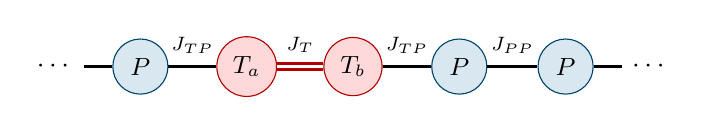
\begin{tikzpicture}[
      P/.style={circle,draw=nanogune!70!black,fill=nanogune!15,minimum size=7mm,font=\small},
      T/.style={circle,draw=red!70!black,fill=red!15,minimum size=7mm,font=\small},
      afm/.style={thick},
      fm/.style={very thick,red!70!black,double,double distance=1pt},
      lbl/.style={font=\scriptsize,midway,above=1pt},
      x=1.35cm]
    \node (l0) at (-0.8,0) {$\cdots$};
    \node[P] (P1) at (0,0) {$P$};
    \node[T] (Ta) at (1,0) {$T_a$};
    \node[T] (Tb) at (2,0) {$T_b$};
    \node[P] (P2) at (3,0) {$P$};
    \node[P] (P3) at (4,0) {$P$};
    \node (r0) at (4.8,0) {$\cdots$};
    \draw[afm] (l0)--(P1);
    \draw[afm] (P1)--(Ta) node[lbl]{$J_{TP}$};
    \draw[fm]  (Ta)--(Tb) node[lbl,black]{$J_{T}$};
    \draw[afm] (Tb)--(P2) node[lbl]{$J_{TP}$};
    \draw[afm] (P2)--(P3) node[lbl]{$J_{PP}$};
    \draw[afm] (P3)--(r0);
  \end{tikzpicture}
  \vspace{1mm}
  \begin{center}
  \begin{tabular}{ccc}
    \toprule
    $J_{PP}$ (AFM) & $J_{TP}$ (AFM) & $J_T$ (FM) \\
    \midrule
    $38$~meV & $40$~meV & $-500$~meV \\
    \bottomrule
  \end{tabular}
  \end{center}
  Since $|J_T|\gg J_{TP},J_{PP}$: each $(T_a,T_b)$ pair freezes into an effective $S=1$ object $\Rightarrow$ mixed $\tfrac12$--$1$--$\tfrac12$ AFM spin chain.
\end{frame}

\begin{frame}{Exact diagonalization: method and scaling}
  \begin{itemize}
    \item $H$ is $SU(2)$-symmetric and one-dimensional $\Rightarrow$ ED gives the numerically exact ground state, spectrum, and total spin $S,S_z$ with no mean-field bias.
    \item Implemented in \texttt{QuTiP}: each spin operator built as a tensor product of Pauli matrices, $H$ assembled bond by bond.
    \item Hilbert space $\dim\mathcal H = 2^{4N}$: $4096$ states at $N=3$, $65536$ at $N=4$.
    \item Dense ED feasible to $n\sim14$--$16$ sites; conserving total $S_z$ + sparse Lanczos/Arnoldi extends this to $n\sim18$--$20$.
  \end{itemize}
\end{frame}

\begin{frame}{Ground-state selection: the Lieb--Mattis theorem}
  \begin{alertblock}{Lieb--Mattis theorem}
    A balanced bipartite chain ($S_A=S_B$) has a total-singlet ($S=0$) ground state for every $N$.
  \end{alertblock}
  \begin{itemize}
    \item $\langle S_z^i\rangle$ vanishes identically in the ground state by symmetry: no local magnetization is visible there.
    \item The intrinsic magnetic texture is instead revealed by the $S_z=+1$ member of the lowest $S=1$ multiplet -- the observable used on the next slide.
  \end{itemize}
\end{frame}

\begin{frame}{ED results: ground state and spin texture ($N=3$)}
  \begin{columns}[c]
    \begin{column}{0.56\textwidth}
      \centering
      
\includegraphics[width=\linewidth]{spin_chain_N3_crop.png}
    \end{column}
    \begin{column}{0.42\textwidth}
      \small
      \begin{itemize}
        \item Ground state: total singlet, $S=0$, $E_0=-514.43$~meV.
        \item Lowest triplet ($S_z{=}{+}1$): large moments on $T_a,T_b$ ($\sim0.13$--$0.23$), small on $P$, alternating sign between successive triangulene units.
        \item Singlet--triplet gap $\Delta = 11.04$~meV.
      \end{itemize}
    \end{column}
  \end{columns}
\end{frame}

\begin{frame}{Part II -- Summary}
  \begin{itemize}
    \item The $P$--$T$--$P$ copolymer is a chemically programmed realization of a mixed $\tfrac12$--$1$--$\tfrac12$ antiferromagnetic Heisenberg chain, with couplings inherited from atomistic MFH/second-order exchange.
    \item MFH spin-density maps and exact-diagonalization spin textures agree qualitatively: the same alternating pattern, from the fully atomistic to the effective spin model.
    \item $S=0$ ground state guaranteed by the Lieb--Mattis theorem; finite singlet--triplet gap ($11.04$~meV at $N=3$) set by $J_{PP}$ and $J_{TP}$.
    \item Linear scaling $n=4N$ of the spin lattice with oligomer length makes the model straightforwardly extensible via sparse ED.
  \end{itemize}
\end{frame}

% =========================================================
\section{Outlook}
% =========================================================

\begin{frame}{Two complementary routes to nanographene magnetism}
  \small
  \begin{columns}[t]
    \begin{column}{0.48\textwidth}
      \textbf{7-AGNR end states}
      \begin{itemize}
        \item Magnetism from topology: $\mathbb Z_2$-protected zero modes at ribbon termini.
        \item Coupling set by ribbon \emph{length} $L$; exponential tunability, $\xi\approx0.38$ monomers.
        \item Validated by Hubbard-dimer superexchange beyond MFH's numerical reach.
      \end{itemize}
    \end{column}
    \begin{column}{0.48\textwidth}
      \textbf{Triangulene--phenalenyl chain}
      \begin{itemize}
        \item Magnetism from chemistry: sublattice-imbalance radicals ($P$,$T$) as designed spin-$\tfrac12$/spin-$1$ units.
        \item Couplings set by \emph{precursor design}; scalable $4N$-site Heisenberg chain.
        \item Validated by exact diagonalization against MFH spin densities.
      \end{itemize}
    \end{column}
  \end{columns}
  \vspace{2mm}
  \begin{block}{Outlook}
    \small Both frameworks combine atomistic MFH with an exactly solvable low-energy model -- a template for engineering length- and chemistry-tunable magnetic couplings for molecular spintronics and quantum information.
  \end{block}
\end{frame}

\begin{frame}[standout]
  Thank you\\
  \vspace{2mm}
  {\large Questions \& discussion}
\end{frame}

\end{document}
